\documentclass[11pt]{amsart}

\usepackage[T1]{fontenc}
\usepackage{lmodern}
\usepackage{amssymb,amsmath}
\usepackage{graphicx}
\usepackage{enumitem}
\usepackage[dvipsnames]{xcolor}
\usepackage[margin=1.15in]{geometry}
\usepackage{xurl}
\usepackage[colorlinks=true,linkcolor=blue!50!black,citecolor=blue!50!black,urlcolor=blue!50!black]{hyperref}

\newtheorem{theorem}{Theorem}[section]
\newtheorem{proposition}[theorem]{Proposition}
\newtheorem{lemma}[theorem]{Lemma}
\newtheorem{corollary}[theorem]{Corollary}
\newtheorem*{shankarthm}{Theorem}
\newtheorem*{shankarconj}{Conjecture}
\theoremstyle{definition}
\newtheorem{definition}[theorem]{Definition}
\theoremstyle{remark}
\newtheorem{remark}[theorem]{Remark}

\numberwithin{equation}{section}

\newcommand{\F}{\mathbb{F}}
\newcommand{\cA}{\mathcal{A}}
\newcommand{\cG}{\mathcal{G}}
\newcommand{\cK}{\mathcal{K}}
\newcommand{\cP}{\mathcal{P}}
\newcommand{\cQ}{\mathcal{Q}}
\newcommand{\Iv}[1]{[\,#1\,]}
\DeclareMathOperator{\wt}{w}
\hypersetup{pdftitle={Even-intersecting families of lattice paths and the Catalan numbers},pdfauthor={Deep Bhattacharjee}}
\providecommand{\doi}[1]{\url{https://doi.org/#1}}

\begin{document}

\title{Even-intersecting families of lattice paths and the Catalan numbers}

\author{Deep Bhattacharjee}
\address{Formerly, Electro-Gravitational Space Propulsion Laboratory (EGSPL),\newline Bhubaneswar, Odisha 751030, India}
\email{d.bhattacharjee@erl-forschung.de}
\email{itsdeep@live.com}
\urladdr{https://orcid.org/0000-0003-0466-750X}
\thanks{Corresponding author: \href{mailto:d.bhattacharjee@erl-forschung.de}{d.bhattacharjee@erl-forschung.de}; ORCID \href{https://orcid.org/0000-0003-0466-750X}{\mbox{0000-0003-0466-750X}}}

\subjclass[2020]{Primary 05A15; Secondary 05D05, 05A05}
\keywords{lattice paths, Eventown theorem, even intersections, Catalan numbers, noncrossing matchings}

\begin{abstract}
Shankar proved that a family of North--East lattice paths from $(0,0)$ to $(n,n)$ in which any two paths share an even number of edges has at most $2^n$ members, and conjectured that exactly $C_n$ families attain this bound, where $C_n$ is the $n$th Catalan number. We prove the conjecture. The proof determines all equality cases of the inequality behind Shankar's bound: they correspond to noncrossing partial matchings of $\{1,\dots,m\}$ whose unmatched points lie under no arc, and there are $\binom{m}{\lfloor m/2\rfloor}$ of them.
\end{abstract}

\maketitle

\section{Introduction}

A lattice path from $(0,0)$ to $(n,n)$ consists of $2n$ unit steps, each north ($N$) or east ($E$). Following Shankar~\cite{Sh}, we say that two such paths intersect in their common edges. The Eventown theorem of Berlekamp~\cite{Be} and Graver~\cite{Gr} bounds families of sets with even pairwise intersections; Shankar proved the following analogue for paths.

\begin{shankarthm}[Shankar {\cite[Theorem~1.4]{Sh}}]
Let $\mathcal F$ be a family of lattice paths from $(0,0)$ to $(n,n)$ in which any two distinct paths have an even number of common edges. Then $|\mathcal F|\le 2^n$.
\end{shankarthm}

The bound is attained by many families. A perfect matching $M$ of $[2n]=\{1,\dots,2n\}$ is \emph{noncrossing} if it contains no two pairs $\{p,q\}$, $\{p',q'\}$ with $p<p'<q<q'$; there are $C_n=\frac1{n+1}\binom{2n}{n}$ of them~\cite{St}. For such $M$ let $\mathcal F_M$ be the set of words $w\in\{E,N\}^{2n}$ with $w_p\ne w_q$ for every pair $\{p,q\}\in M$. Each pair can be filled with $EN$ or $NE$ independently, so $|\mathcal F_M|=2^n$, and every word in $\mathcal F_M$ has $n$ letters of each kind, so it describes a path from $(0,0)$ to $(n,n)$. Shankar showed that any two paths of $\mathcal F_M$ have an even number of common edges and that different matchings give different families~\cite[Section~4]{Sh}; Figure~\ref{fig:families} shows the two families for $n=2$. He conjectured that there are no other extremal families.

\begin{shankarconj}[Shankar {\cite[Conjecture~4.1]{Sh}}]
There are exactly $C_n$ families of $2^n$ lattice paths from $(0,0)$ to $(n,n)$ in which every two distinct paths have an even number of common edges.
\end{shankarconj}

Shankar verified the conjecture for $n\le5$. We prove it.

\begin{theorem}\label{thm:shankar}
Let $\mathcal F$ be a family of $2^n$ lattice paths from $(0,0)$ to $(n,n)$ in which every two distinct paths have an even number of common edges. Then $\mathcal F=\mathcal F_M$ for a noncrossing perfect matching $M$ of $[2n]$. In particular, Shankar's conjecture holds.
\end{theorem}

\begin{figure}[ht]
\centering
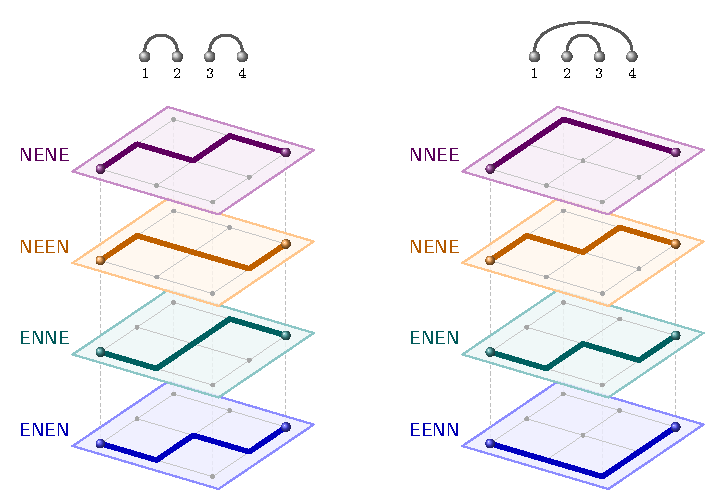
\includegraphics[width=0.86\textwidth]{figures/families}
\caption{The two extremal families for $n=2$. On the left $M=\{\{1,2\},\{3,4\}\}$, on the right $M=\{\{1,4\},\{2,3\}\}$; each family has four paths, drawn on four parallel copies of the grid $\{0,1,2\}^2$. Each pair of paths in a family shares $0$ or $2$ edges.}
\label{fig:families}
\end{figure}

Shankar's proof reduces the bound to an inequality for collections of sets of binary words~\cite[Lemma~2.3]{Sh}, proved by induction on the length of the words. Theorem~\ref{thm:shankar} follows from a description of all collections for which this inequality is an equality, and we now state it. Identify $N$ with $1$ and $E$ with $0$, so that a path with $m$ steps becomes a word in $L(m)=\{0,1\}^m$. For $x\in L(m)$ write $\wt(x)$ for the number of letters $1$ in $x$, its \emph{weight}, and $x_{<i}=x_1\cdots x_{i-1}$. For $x,y\in L(m)$ let
\[
B_m(x,y)=\#\{i\in[m]:\ x_i=y_i\ \text{and}\ \wt(x_{<i})=\wt(y_{<i})\}\bmod 2\ \in\F_2 .
\]
By~\eqref{eq:common} below, $B_m(x,y)$ is the parity of the number of common edges of the two paths.

An \emph{admissible system of length $m$} is a finite collection $\cA$ of pairwise disjoint nonempty subsets of $L(m)$, its \emph{classes}, such that
\begin{enumerate}[label=\textup{(A\arabic*)}]
\item all words in a class have the same weight;
\item $B_m(x,y)=m$ in $\F_2$ whenever $x$ and $y$ lie in the same class;
\item for distinct classes $A$ and $A'$, $B_m$ is constant on $A\times A'$.
\end{enumerate}

Shankar's Lemma~2.3 states that $\sum_{A\in\cA}|A|^2\le 2^m$ for every admissible system $\cA$ of length $m$; we reprove it as Proposition~\ref{prop:inequality}, because its equality case is our starting point. We call $\cA$ \emph{extremal} if $\sum_{A\in\cA}|A|^2=2^m$.

The extremal systems come from noncrossing partial matchings. A \emph{skeleton} of $[m]$ is a pair $(M,S)$, where $M$ is a set of pairwise disjoint two-element subsets of $[m]$, the \emph{arcs}, and $S=[m]\setminus\bigcup M$ is the set of \emph{free points}, such that
\begin{enumerate}[label=(\alph*)]
\item no two arcs cross: there are no arcs $\{p,q\}$, $\{p',q'\}$ with $p<p'<q<q'$;
\item no free point lies under an arc: there are no $s\in S$ and $\{p,q\}\in M$ with $p<s<q$.
\end{enumerate}
Let $s_1<\dots<s_k$ be the free points. For $a\in L(k)$ the class $C_a=C_a(M,S)$ consists of the words $x\in L(m)$ with $x_p\ne x_q$ for every arc $\{p,q\}$ and $x_{s_j}=a_j$ for $1\le j\le k$. The \emph{skeleton system} of $(M,S)$ is
\[
\Sigma(M,S)=\{C_a(M,S):\ a\in L(k)\}.
\]
Figure~\ref{fig:skeleton} shows a skeleton of $[11]$.

\begin{theorem}\label{thm:main}
An admissible system of length $m$ is extremal if and only if it is a skeleton system $\Sigma(M,S)$ of a skeleton $(M,S)$ of $[m]$. Different skeletons of $[m]$ give different skeleton systems.
\end{theorem}

\begin{corollary}\label{cor:count}
For every $m\ge0$ there are exactly $\binom{m}{\lfloor m/2\rfloor}$ extremal admissible systems of length $m$.
\end{corollary}

A family $\mathcal F$ as in Theorem~\ref{thm:shankar} is an extremal admissible system of length $2n$ with a single class, and Theorem~\ref{thm:main} forces such a system to be $\Sigma(M,\varnothing)=\{\mathcal F_M\}$; Section~\ref{sec:final} gives the details.

The proof of Theorem~\ref{thm:main} follows Shankar's induction, which deletes the last letter of every word. In Section~\ref{sec:induction} we show that for an extremal system the two systems of length $m-1$ produced by the induction coincide, so that by induction they form one skeleton system, and the system of length $m$ is obtained from it by grouping some of its classes in pairs. Section~\ref{sec:star} proves a rigidity statement, Lemma~\ref{lem:star}, for two words of adjacent weights that are indistinguishable from all words of other weights; it rests on the effect of moving a path across one unit square. In Section~\ref{sec:groupings} we use it to show that only two groupings are possible, and each gives a skeleton system of length $m$. Corollary~\ref{cor:count} then follows from a bijection between skeletons and nonnegative $\pm1$ sequences.

\begin{figure}[ht]
\centering
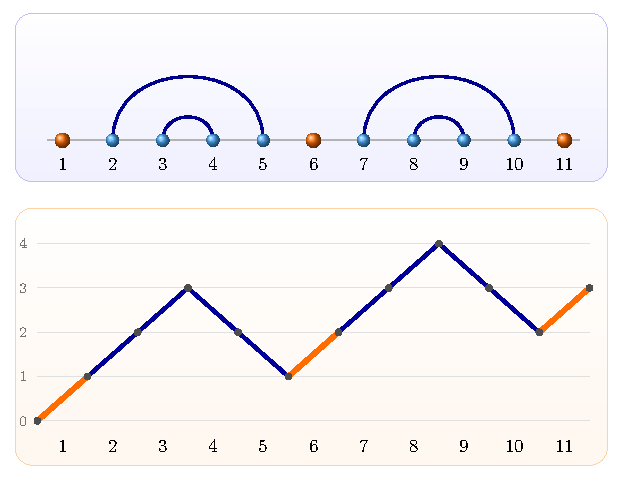
\includegraphics[width=0.8\textwidth]{figures/skeleton}
\caption{Top: the skeleton of $[11]$ with arcs $\{2,5\},\{3,4\},\{7,10\},\{8,9\}$ and free points $1,6,11$. Its system has $2^3$ classes of $2^4$ words; for example $C_{101}$ consists of the words $1\,x_2x_3\bar x_3\bar x_2\,0\,x_7x_8\bar x_8\bar x_7\,1$, where $\bar x=1-x$. Bottom: the nonnegative $\pm1$ sequence attached to it in Section~\ref{sec:final}; free points and left ends of arcs are up steps.}
\label{fig:skeleton}
\end{figure}

\section{Words, paths and skeletons}\label{sec:skeletons}

For a word $x\in L(m)$ the $i$th step of its path starts at the point $(i-1-\wt(x_{<i}),\wt(x_{<i}))$ and goes north if $x_i=1$ and east if $x_i=0$. A point $(u,v)$ has \emph{level} $u+v$, so the $i$th step of every path starts at level $i-1$. Two steps can therefore be the same edge only if they have the same index $i$, and then they are the same edge exactly when they start at the same point and go in the same direction. Writing $E(x)$ for the set of edges of the path of $x$, we get
\begin{equation}\label{eq:common}
|E(x)\cap E(y)|=\#\{i\in[m]:\ x_i=y_i\ \text{and}\ \wt(x_{<i})=\wt(y_{<i})\},
\end{equation}
so $B_m(x,y)\equiv|E(x)\cap E(y)|\pmod 2$. Throughout, $\Iv{P}\in\F_2$ is $1$ if the statement $P$ holds and $0$ otherwise, and for a set $X\subseteq L(m-1)$ and $e\in\{0,1\}$ we write $Xe=\{xe:\ x\in X\}\subseteq L(m)$.

\begin{lemma}\label{lem:basic}
\textup{(a)} $B_m(x,x)=m$ for every $x\in L(m)$.

\textup{(b)} For $x,y\in L(m-1)$ and $e,e'\in\{0,1\}$,
\[
B_m(xe,ye')=B_{m-1}(x,y)+\Iv{e=e'}\,\Iv{\wt(x)=\wt(y)} .
\]
\end{lemma}

\begin{proof}
In (a) every position counts. In (b) the first $m-1$ positions contribute $B_{m-1}(x,y)$, and the last one counts exactly when $e=e'$ and $\wt(x)=\wt(y)$.
\end{proof}

A subcollection of an admissible system is again admissible, and the empty collection is admissible.

\begin{proposition}\label{prop:skeleton}
Let $(M,S)$ be a skeleton of $[m]$ with $k$ free points, and let $a,a'\in L(k)$, $x\in C_a$ and $y\in C_{a'}$. Then
\[
\wt(x)=|M|+\wt(a)\qquad\text{and}\qquad B_m(x,y)=B_k(a,a').
\]
Consequently $\Sigma(M,S)$ is an extremal admissible system of length $m$, and the skeleton $(M,S)$ can be recovered from $\Sigma(M,S)$.
\end{proposition}

\begin{proof}
Each arc carries one letter $1$, so $\wt(x)=|M|+\wt(a)$. Put $\Delta_i=\wt(x_{<i})-\wt(y_{<i})$, so that position $i$ counts in $B_m(x,y)$ when $x_i=y_i$ and $\Delta_i=0$.

Let $s=s_j$ be a free point. By condition (b), every arc lies entirely before $s$ or entirely after it, and each arc before $s$ contributes one letter $1$ to $x_{<s}$ and to $y_{<s}$. Hence $\Delta_s=\wt(a_{<j})-\wt(a'_{<j})$, and since $x_s=a_j$ and $y_s=a'_j$, position $s$ counts in $B_m(x,y)$ exactly when position $j$ counts in $B_k(a,a')$.

Let $\{p,q\}$ be an arc with $p<q$. By conditions (a) and (b), the positions strictly between $p$ and $q$ are covered by arcs that lie strictly between $p$ and $q$, and each of them adds one letter $1$ to $x$ and one to $y$. So $\Delta_q=\Delta_p+x_p-y_p$. If $x_p=y_p$, then $x_q=y_q$ and $\Delta_q=\Delta_p$, so positions $p$ and $q$ both count or both do not. If $x_p\ne y_p$, then $x_q\ne y_q$ and neither counts. In either case the arc contributes an even number. Adding up the contributions gives $B_m(x,y)=B_k(a,a')$.

The classes $C_a$ are nonempty, pairwise disjoint and of size $2^{|M|}$. By the two identities, the words of $C_a$ have weight $|M|+\wt(a)$, $B_m$ is constant on $C_a\times C_{a'}$, and on $C_a\times C_a$ it equals $B_k(a,a)=k=m-2|M|$ by Lemma~\ref{lem:basic}(a), which is $m$ in $\F_2$. So $\Sigma(M,S)$ is admissible, and $\sum_a|C_a|^2=2^k\cdot 4^{|M|}=2^m$.

Finally, let $U$ be the union of the classes. Two positions $p\ne q$ satisfy $x_p\ne x_q$ for all $x\in U$ exactly when $\{p,q\}\in M$: if $p$ and $q$ lie on different arcs, or one of them is free, the letters at $p$ and $q$ can be chosen independently and in particular equal. So $U$ determines $M$, and $S$ is the complement of $\bigcup M$.
\end{proof}

\section{The induction step}\label{sec:induction}

In this section $\cA=\{A_1,\dots,A_r\}$ is an admissible system of length $m\ge1$. For $1\le i\le r$ and $e\in\{0,1\}$ let
\[
B_i^e=\{x\in L(m-1):\ xe\in A_i\},
\]
so that $A_i=B_i^0 0\cup B_i^1 1$. Let $I$ be the set of indices $i$ with $B_i^0\ne\varnothing$ and $B_i^1\ne\varnothing$, and following Shankar put
\[
\cG_0=\{B_i^0:\ B_i^0\ne\varnothing\}\cup\{B_i^1:\ i\in I\},\qquad
\cG_1=\{B_i^1:\ B_i^1\ne\varnothing\}\cup\{B_i^0:\ i\in I\}.
\]
For a collection $\mathcal X$ of finite sets write $\|\mathcal X\|=\sum_{X\in\mathcal X}|X|^2$.

\begin{lemma}\label{lem:disjoint}
If $B_i^0\cap B_j^1\ne\varnothing$, then $i\ne j$, $B_i^1=\varnothing$ and $B_j^0=\varnothing$.
\end{lemma}

\begin{proof}
Let $u\in B_i^0\cap B_j^1$, so $u0\in A_i$ and $u1\in A_j$. These words have different weights, so $i\ne j$ by (A1). By Lemma~\ref{lem:basic}, $B_m(u0,u1)=B_{m-1}(u,u)=m-1$.

Suppose $v1\in A_i$. By (A2), $m=B_m(u0,v1)=B_{m-1}(u,v)$. Since $v1$ and $u0$ have the same weight, $\wt(v)=\wt(u)-1$, so Lemma~\ref{lem:basic} gives $B_m(u1,v1)=B_{m-1}(u,v)=m$. Now $u0,v1\in A_i$ and $u1\in A_j$, so (A3) gives $m=B_m(v1,u1)=B_m(u0,u1)=m-1$, a contradiction. Hence $B_i^1=\varnothing$.

Suppose $v0\in A_j$. By (A2), $m=B_m(u1,v0)=B_{m-1}(u,v)$, and $\wt(v)=\wt(u)+1$, so $B_m(u0,v0)=B_{m-1}(u,v)=m$. Since $u1,v0\in A_j$ and $u0\in A_i$, (A3) gives $m=B_m(u0,v0)=B_m(u0,u1)=m-1$, again a contradiction. Hence $B_j^0=\varnothing$.
\end{proof}

\begin{proposition}[{Shankar~\cite[Lemma~2.3]{Sh}}]\label{prop:inequality}
The sets listed in $\cG_0$ are nonempty and pairwise disjoint, $\cG_0$ is an admissible system of length $m-1$, and the same holds for $\cG_1$. Moreover
\[
\|\cA\|\le\|\cG_0\|+\|\cG_1\| ,
\]
with equality if and only if $|B_i^0|=|B_i^1|$ for every $i\in I$. Consequently $\|\cA\|\le 2^m$, and if $\cA$ is extremal, then $\cG_0$ and $\cG_1$ are extremal and $|B_i^0|=|B_i^1|$ for every $i\in I$.
\end{proposition}

\begin{proof}
We treat $\cG_0$; the case of $\cG_1$ is symmetric. Sets $B_i^0$ and $B_j^0$ with $i\ne j$ are disjoint because $A_i$ and $A_j$ are, and the same holds for $B_i^1$ and $B_j^1$. If $B_i^0\cap B_j^1\ne\varnothing$ with $j\in I$, then Lemma~\ref{lem:disjoint} gives $B_j^0=\varnothing$, which contradicts $j\in I$. So the sets of $\cG_0$ are pairwise disjoint.

Each set of $\cG_0$ lies in one weight level, since $\wt(x)=\wt(A_i)-e$ for $x\in B_i^e$. For $x,y\in B_i^e$, Lemma~\ref{lem:basic} and (A2) give $m=B_m(xe,ye)=B_{m-1}(x,y)+1$, so $B_{m-1}(x,y)=m-1$. For $x\in B_i^e$ and $y\in B_j^{e'}$ in two different sets of $\cG_0$,
\[
B_{m-1}(x,y)=B_m(xe,ye')+\Iv{e=e'}\,\Iv{\wt(x)=\wt(y)} .
\]
The last term depends only on $i,j,e,e'$, and $B_m(xe,ye')$ is constant on $A_i\times A_j$ by (A3) when $i\ne j$, and equals $m$ by (A2) when $i=j$ (then $\{e,e'\}=\{0,1\}$). So $B_{m-1}$ is constant on the product of any two distinct sets of $\cG_0$, and $\cG_0$ is admissible.

For $i\notin I$ one of $B_i^0$, $B_i^1$ is empty, so $|A_i|^2=|B_i^0|^2+|B_i^1|^2$. For $i\in I$,
\[
|A_i|^2=(|B_i^0|+|B_i^1|)^2\le 2|B_i^0|^2+2|B_i^1|^2 ,
\]
with equality if and only if $|B_i^0|=|B_i^1|$. Summing over $i$ gives $\|\cA\|\le\|\cG_0\|+\|\cG_1\|$ with the stated equality case. The bound $\|\cA\|\le2^m$ follows by induction on $m$; for $m=0$ the set $L(0)$ has one element, so $\|\cA\|\le1$. If $\|\cA\|=2^m$, then $2^m\le\|\cG_0\|+\|\cG_1\|\le 2^{m-1}+2^{m-1}$ forces equality everywhere.
\end{proof}

Let $Z$ be the set of indices with $B_i^1=\varnothing$ and $O$ the set of indices with $B_i^0=\varnothing$, so that $[r]$ is the disjoint union of $I$, $Z$ and $O$. Put
\[
\cK=\{B_i^0,\ B_i^1:\ i\in I\},\qquad \cP=\{B_i^0:\ i\in Z\},\qquad \cQ=\{B_j^1:\ j\in O\},
\]
so that $\cG_0=\cK\cup\cP$ and $\cG_1=\cK\cup\cQ$. By Proposition~\ref{prop:inequality} the sets of $\cK\cup\cP$ are pairwise disjoint, and so are those of $\cK\cup\cQ$; a set of $\cP$ may meet a set of $\cQ$.

\begin{lemma}\label{lem:merge}
If $\cA$ is extremal, then $\cP=\cQ$, and hence $\cG_0=\cG_1$.
\end{lemma}

\begin{proof}
Consider the bipartite graph $H$ with vertex classes $\cP$ and $\cQ$, in which $P\in\cP$ and $Q\in\cQ$ are adjacent when $P\cap Q\ne\varnothing$. For a connected component $\Gamma$ of $H$ let $U_\Gamma$ be the union of the sets in $\Gamma$. We claim that
\[
\cK\cup\{U_\Gamma:\ \Gamma\text{ a component of }H\}
\]
is an admissible system of length $m-1$.

The sets $U_\Gamma$ are nonempty, disjoint from each other because sets in different components do not meet, and disjoint from the sets of $\cK$. Adjacent sets share a word, so all sets in a component lie in one weight level, and (A1) holds.

We first show that for any two sets $X,Y$ of $\cK\cup\cP\cup\cQ$, not both in $\cK$, $B_{m-1}$ is constant on $X\times Y$. If $X$ and $Y$ both lie in $\cG_0$ or both in $\cG_1$, this follows from the admissibility of $\cG_0$ or $\cG_1$ (when $X=Y$ the constant is $m-1$). Otherwise one of them is some $B_i^0$ with $i\in Z$ and the other some $B_j^1$ with $j\in O$; then $i\ne j$, and Lemma~\ref{lem:basic} gives $B_{m-1}(x,y)=B_m(x0,y1)$ for $x\in B_i^0$, $y\in B_j^1$, which is constant by (A3). Let $c(X,Y)$ denote the constant. If $X$ and $X'$ share a word $z$, then $c(X,Y)=B_{m-1}(z,y)=c(X',Y)$ for any $y\in Y$. Consequently, for $X\in\cK$ and a component $\Gamma$, $c(X,Y)$ is the same for all $Y\in\Gamma$, so $B_{m-1}$ is constant on $X\times U_\Gamma$; and for distinct components $\Gamma,\Gamma'$ it is constant on $U_\Gamma\times U_{\Gamma'}$. This gives (A3).

For (A2), let $X,Y\in\Gamma$; we show $c(X,Y)=m-1$ by induction on the distance $t$ between $X$ and $Y$ in $H$. If $t=0$ this is (A2) for $\cG_0$ or $\cG_1$. If $t=1$, pick $z\in X\cap Y$; then $c(X,Y)=B_{m-1}(z,z)=m-1$. If $t\ge2$, take a shortest path $X=X_0,X_1,\dots,X_t=Y$ and words $z\in X_0\cap X_1$, $z'\in X_{t-1}\cap X_t$. Then $c(X,Y)=B_{m-1}(z,z')=c(X_1,X_{t-1})$, and $X_1$, $X_{t-1}$ are at distance $t-2$.

By Proposition~\ref{prop:inequality} applied to this system, and since $\cG_0$ is extremal,
\[
\|\cK\|+\sum_\Gamma|U_\Gamma|^2\le 2^{m-1}=\|\cK\|+\sum_\Gamma\sum_{P\in\Gamma\cap\cP}|P|^2 .
\]
The sets of $\cP$ in one component are disjoint, so $|U_\Gamma|^2\ge\bigl(\sum_{P\in\Gamma\cap\cP}|P|\bigr)^2\ge\sum_{P\in\Gamma\cap\cP}|P|^2$ for each $\Gamma$. Hence all these inequalities are equalities. In the same way, using $\cG_1$, $|U_\Gamma|^2=\bigl(\sum_{Q\in\Gamma\cap\cQ}|Q|\bigr)^2=\sum_{Q\in\Gamma\cap\cQ}|Q|^2$. A component without sets of $\cQ$ would give $|U_\Gamma|^2=0$, which is impossible, and likewise every component contains a set of $\cP$. Since the sets are nonempty, $\bigl(\sum|P|\bigr)^2=\sum|P|^2$ forces $\Gamma$ to contain exactly one set $P$ of $\cP$, and then $U_\Gamma=P$; likewise $\Gamma$ contains exactly one set $Q$ of $\cQ$ and $U_\Gamma=Q$. So every component consists of two equal sets $P=Q$, and $\cP=\cQ$.
\end{proof}

The structure of an extremal system is now described by a pairing of the classes of $\cG_0$. We record it in terms of the index words of a skeleton system.

\begin{definition}\label{def:grouping}
Let $k\ge0$. A \emph{grouping} of $L(k)$ is a partition of $L(k)$ into singletons $\{c\}$ and ordered pairs $(a,b)$ with $a\ne b$. Its \emph{items} are $(a,0)$ and $(b,1)$ for each pair $(a,b)$, and $(c,0)$ and $(c,1)$ for each singleton $\{c\}$. For $a,b,c\in L(k)$ put $f_{a,b}(c)=B_k(a,c)+B_k(b,c)$. The grouping is \emph{admissible} if
\begin{enumerate}[label=\textup{(G\arabic*)}]
\item $\wt(a)=\wt(b)+1$ and $B_k(a,b)=k+1$ for every pair $(a,b)$;
\item for every pair $(a,b)$ and every item $(c,e)$ with $c\notin\{a,b\}$,
\[
f_{a,b}(c)=\Iv{e=0}\,\Iv{\wt(c)=\wt(a)}+\Iv{e=1}\,\Iv{\wt(c)=\wt(b)} .
\]
\end{enumerate}
\end{definition}

If $\{c\}$ is a singleton of an admissible grouping and $(a,b)$ a pair, then (G2) for the items $(c,0)$ and $(c,1)$ gives $\Iv{\wt(c)=\wt(a)}=f_{a,b}(c)=\Iv{\wt(c)=\wt(b)}$. As $\wt(a)\ne\wt(b)$, both sides vanish:
\begin{enumerate}[label=\textup{(G3)}]
\item a singleton $\{c\}$ has $\wt(c)\notin\{\wt(a),\wt(b)\}$ and $f_{a,b}(c)=0$, for every pair $(a,b)$.
\end{enumerate}

\begin{lemma}\label{lem:grouping}
Let $\cA$ be extremal and suppose that $\cG_0=\Sigma(M',S')$ for a skeleton $(M',S')$ of $[m-1]$ with $k$ free points. Write $C_a=C_a(M',S')$. Then there is an admissible grouping of $L(k)$ such that the classes of $\cA$ are the sets $C_a0\cup C_b1$ for the pairs $(a,b)$, and the sets $C_c0$ and $C_c1$ for the singletons $\{c\}$.
\end{lemma}

\begin{proof}
By Lemma~\ref{lem:merge}, $\cG_0=\cK\cup\cP$ with $\cP=\cQ$, and the sets of $\cK\cup\cP$ are pairwise disjoint. For $i\in I$ write $B_i^0=C_a$ and $B_i^1=C_b$, and make $(a,b)$ a pair; then $A_i=C_a0\cup C_b1$. Every class $C_c$ in $\cP=\cQ$ equals $B_i^0$ for exactly one $i\in Z$ and $B_j^1$ for exactly one $j\in O$, so $A_i=C_c0$ and $A_j=C_c1$; make $\{c\}$ a singleton. This is a partition of $L(k)$, and every class of $\cA$ arises once.

By Proposition~\ref{prop:skeleton}, words of $C_a$ have weight $|M'|+\wt(a)$, and $B_{m-1}(x,y)=B_k(a,a')$ for $x\in C_a$, $y\in C_{a'}$. Note $m-1=k+2|M'|$. For a pair $(a,b)$, (A1) for $A_i=C_a0\cup C_b1$ gives $\wt(a)=\wt(b)+1$, and (A2) with Lemma~\ref{lem:basic} gives $B_k(a,b)=B_m(x0,y1)=m=k+1$ for $x\in C_a$, $y\in C_b$. This is (G1).

For (G2), let $(a,b)$ be a pair and $(c,e)$ an item with $c\notin\{a,b\}$, and let $A'$ be the class of $\cA$ that contains $C_ce$. Then $A'\ne C_a0\cup C_b1$, so by (A3) $B_m$ takes the same value at $(x0,z e)$ and at $(y1,ze)$ for $x\in C_a$, $y\in C_b$, $z\in C_c$. By Lemma~\ref{lem:basic} these values are $B_k(a,c)+\Iv{e=0}\Iv{\wt(c)=\wt(a)}$ and $B_k(b,c)+\Iv{e=1}\Iv{\wt(c)=\wt(b)}$, and their equality is (G2).
\end{proof}

\section{A rigidity lemma for pairs of words}\label{sec:star}

The heart of the proof is the following lemma. For $j\ge1$ write $(10)^j$ for the word $10\cdots10$ of length $2j$, and similarly $(01)^j$.

\begin{lemma}\label{lem:star}
Let $k\ge1$ and $a,b\in L(k)$ with $\wt(a)=\wt(b)+1$ and $B_k(a,b)=k+1$, and suppose that $B_k(a,c)=B_k(b,c)$ for every $c\in L(k)$ with $\wt(c)\notin\{\wt(a),\wt(b)\}$. Then either $a=u1$ and $b=u0$ for some $u\in L(k-1)$, or $k=2j+1\ge3$ is odd and
\[
a=1(10)^j,\qquad b=0(01)^j .
\]
\end{lemma}

The second case cannot be excluded from the hypotheses alone: for $k=3$ the pair $a=110$, $b=001$ satisfies them, as the computation for $k=3$ below shows. Section~\ref{sec:groupings} removes it by a separate argument.

For $p\in L(k)$ and $0\le\ell\le k$ let $\pi_p(\ell)=(\ell-\wt(p_{\le\ell}),\wt(p_{\le\ell}))$, where $p_{\le\ell}=p_1\cdots p_\ell$, be the point the path of $p$ reaches after $\ell$ steps. It is the only point of the path at level $\ell$. Let $V_p$ be the indicator function of the set of these points. For a lattice point $v=(x,y)$ let $Q_v$ be the unit square with lower left corner $v$, and let $\partial Q_v$ be the set of its four sides.

\begin{lemma}\label{lem:cell}
Let $p\in L(k)$ and let $v$ be a lattice point of level $\ell\le k-2$. Then
\[
|E(p)\cap\partial Q_v|=V_p(v)+V_p\bigl(v+(1,1)\bigr).
\]
If $c\in L(k)$ passes through $v$ and $v+(1,1)$ and $c'$ is obtained from $c$ by exchanging the letters in positions $\ell+1$ and $\ell+2$, then $B_k(p,c)+B_k(p,c')=V_p(v)+V_p(v+(1,1))$ in $\F_2$.
\end{lemma}

\begin{proof}
The bottom and left sides of $Q_v$ start at $v$. If the path of $p$ visits $v$, it leaves $v$ along exactly one of them, because $v$ has level $\ell<k$; otherwise it uses neither. The top and right sides end at $v+(1,1)$, and the path uses exactly one of them if it visits $v+(1,1)$ and neither otherwise. This proves the first identity. For the second, $c$ and $c'$ agree outside the positions $\ell+1$ and $\ell+2$, where one of them reads $01$ and the other $10$; so their paths go around $Q_v$ on opposite sides and $E(c)$ and $E(c')$ differ exactly in $\partial Q_v$. Hence $|E(p)\cap E(c)|+|E(p)\cap E(c')|\equiv|E(p)\cap\partial Q_v|\pmod2$, and~\eqref{eq:common} finishes the proof.
\end{proof}

\begin{figure}[ht]
\centering
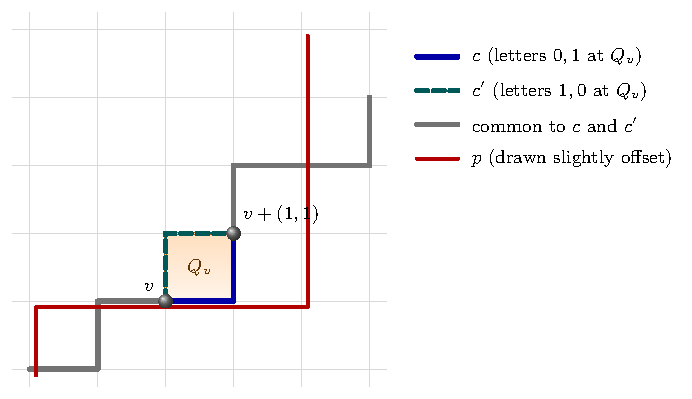
\includegraphics[width=0.62\textwidth]{figures/cellflip}
\caption{Lemma~\ref{lem:cell}. The words $c$ and $c'$ differ in two consecutive letters, so their paths go around the square $Q_v$ on opposite sides and their edge sets differ by the four sides of $Q_v$. A path $p$ through $v$ uses one side at $v$ and, if it passes through $v+(1,1)$, one side there.}
\label{fig:cellflip}
\end{figure}

\begin{proof}[Proof of Lemma~\ref{lem:star}]
For $c\in L(k)$ put $f(c)=B_k(a,c)+B_k(b,c)$, so that $f(c)=0$ whenever $\wt(c)\notin\{\wt(a),\wt(b)\}$. For $e\in\{0,1\}$ and $p\in L(k)$ let $\lambda_e(p)$ be the length of the initial run of letters $e$ in $p$. The path of $0^k=0\cdots0$ runs along the $x$-axis, so by~\eqref{eq:common}
\begin{equation}\label{eq:runs}
B_k(p,0^k)=\lambda_0(p),\qquad B_k(p,1^k)=\lambda_1(p)\qquad\text{in }\F_2 .
\end{equation}

\emph{Small $k$.} For $k=1$ the only pair is $a=1$, $b=0$, which is of the first kind with $u$ empty. For $k=2$ we need $B_2(a,b)=1$. If $\wt(b)=0$, then $b=00$ and $a\in\{01,10\}$, and $B_2(10,00)=0$, $B_2(01,00)=1$; so $(a,b)=(01,00)$. If $\wt(b)=1$, then $a=11$, and $B_2(11,01)=0$, $B_2(11,10)=1$; so $(a,b)=(11,10)$. For $k=3$ we need $B_3(a,b)=0$, and the words $000$ and $111$ can serve as $c$ unless their weight is $\wt(a)$ or $\wt(b)$. If $\wt(b)=0$, then $b=000$ and $B_3(a,b)=\lambda_0(a)$ by~\eqref{eq:runs}, so $a\in\{100,001\}$; and $a=100$ fails at $c=111$, because $f(111)=\lambda_1(100)+\lambda_1(000)=1$. So $(a,b)=(001,000)$. The case $\wt(b)=2$ is symmetric under exchanging the letters $0$ and $1$ and reversing the roles of $a$ and $b$; it leaves $(a,b)=(111,110)$. If $\wt(b)=1$, both $000$ and $111$ are available, so $\lambda_0(a)\equiv\lambda_0(b)$ and $\lambda_1(a)\equiv\lambda_1(b)$. The pairs $(\lambda_0,\lambda_1)\bmod 2$ of $110,101,011$ are $(0,0),(0,1),(1,0)$ and those of $100,010,001$ are $(0,1),(1,0),(0,0)$, which leaves the pairs $(101,100)$, $(011,010)$ and $(110,001)$; all three have $B_3(a,b)=0$. The first two are of the first kind and the third is $1(10)^1,0(01)^1$.

From now on $k\ge4$. Let $J=V_a+V_b$ in $\F_2$. At each level $a$ and $b$ have one point each, so $J$ takes the value $1$ at exactly two points of a level where $a$ and $b$ are apart and vanishes on the levels where they meet; in particular $J(0,0)=0$.

\emph{Testable points.} Call a lattice point $v=(x,y)$ of level $\ell\le k-2$ \emph{testable} if some word $c$ of weight outside $\{\wt(a),\wt(b)\}$ passes through $v$ and $v+(1,1)$. For such $v$ the word $c'$ of Lemma~\ref{lem:cell} has the same weight as $c$, so $f(c)=f(c')=0$, and adding the identities of Lemma~\ref{lem:cell} for $p=a$ and $p=b$ gives
\begin{equation}\label{eq:diag}
J(v)=J\bigl(v+(1,1)\bigr)\qquad\text{for every testable }v .
\end{equation}
A word through $v$ and $v+(1,1)$ has $y+1$ letters $1$ among its first $\ell+2$ letters and $k-\ell-2$ further letters, so its weight can be any $t$ with $y+1\le t\le k-x-1$, an interval of $k-\ell-1$ integers. Since $\{\wt(a),\wt(b)\}=\{\wt(b),\wt(b)+1\}$, we get:
\begin{enumerate}[label=\textup{(T\arabic*)}]
\item every point of level $\ell\le k-4$ is testable;
\item a point $(x,y)$ of level $k-3$ is testable unless $y=\wt(b)-1$.
\end{enumerate}

\emph{Diagonals.} For $\ell\le k-2$ let $D_\ell$ be the set of differences $x-y$ over the points $(x,y)$ of level $\ell$ with $J(x,y)=1$. Then $D_\ell$ has $0$ or $2$ elements, all of the parity of $\ell$ and in $[-\ell,\ell]$, and $D_0=\varnothing$. For $\ell\le k-4$ and $|d|\le\ell$, the point of level $\ell+2$ with difference $d$ is $v+(1,1)$ for the point $v$ of level $\ell$ with difference $d$, so (T1) and~\eqref{eq:diag} give
\begin{equation}\label{eq:D}
D_{\ell+2}\cap[-\ell,\ell]=D_\ell\qquad(0\le\ell\le k-4).
\end{equation}
Suppose $\ell_0\le k-2$ is the smallest level of a given parity with $D_{\ell_0}\ne\varnothing$, and $\ell_0\ge2$. By~\eqref{eq:D}, $D_{\ell_0}\cap[-(\ell_0-2),\ell_0-2]=\varnothing$, so $D_{\ell_0}=\{\ell_0,-\ell_0\}$: the two paths are at $(\ell_0,0)$ and $(0,\ell_0)$, so one word begins with $\ell_0$ letters $0$ and the other with $\ell_0$ letters $1$, and the paths are apart at every level $1,\dots,\ell_0$. As $D_{\ell_0-2}=\varnothing$, this is possible only for $\ell_0=2$, and then $D_1\ne\varnothing$. Applying this to both parities, and using~\eqref{eq:D} to propagate, we find three cases.
\begin{enumerate}[label=(\Roman*)]
\item $a_1=b_1$. Then $D_1=\varnothing$, so also $D_2=\varnothing$, and $D_\ell=\varnothing$ for all $\ell\le k-2$: the words $a$ and $b$ agree in their first $k-2$ letters.
\item $a_1\ne b_1$ and $D_\ell=\varnothing$ for every even $\ell\le k-2$. Then the paths are apart at level $1$ and meet at level $2$, necessarily at $(1,1)$: one word begins with $10$ and the other with $01$.
\item $a_1\ne b_1$ and $D_2\ne\varnothing$. Then $D_1=\{1,-1\}$ and $D_2=\{2,-2\}$, and by~\eqref{eq:D} $D_\ell=\{1,-1\}$ for odd $\ell\le k-2$ and $D_\ell=\{2,-2\}$ for even $2\le\ell\le k-2$.
\end{enumerate}

\emph{Case} (I). Let $t$ be the first position where $a$ and $b$ differ; then $t\in\{k-1,k\}$. If $t=k-1$, then the first $k-2$ positions count in $B_k(a,b)$, position $k-1$ does not, and position $k$ does not either, because $\wt(a_{<k})\ne\wt(b_{<k})$. So $B_k(a,b)=k-2=k$ in $\F_2$, contrary to the hypothesis $B_k(a,b)=k+1$. Hence $t=k$, and $\wt(a)=\wt(b)+1$ gives $a=u1$ and $b=u0$ with $u=a_{<k}$.

\emph{Case} (II). Both words contain a letter $1$ among their first two letters, so $\wt(a),\wt(b)\ge1$ and $c=0^k$ is admissible in the hypothesis. By~\eqref{eq:runs}, $f(0^k)=\lambda_0(a)+\lambda_0(b)=0+1=1$, a contradiction.

\emph{Case} (III), $k$ even. The paths are apart at every level from $1$ to $k-2$. At level $k-2$ their differences are $2$ and $-2$, so at level $k-1$ they are in $\{1,3\}$ and $\{-3,-1\}$, and the paths are apart there too. Hence no position $i\ge2$ counts in $B_k(a,b)$, and position $1$ does not count because $a_1\ne b_1$. So $B_k(a,b)=0$, while $k+1=1$ in $\F_2$, a contradiction.

\emph{Case} (III), $k=2j+1$ odd. Then $j\ge2$. Let $p^+$ be the one of $a,b$ whose path has difference $+2$ at level $2$, and $p^-$ the other. Following the differences $1,2,1,2,\dots$ level by level, $p^+$ is at $(i+1,i)$ at level $2i+1$ and at $(i+1,i-1)$ at level $2i$, for every level from $1$ to $k-2$; so its first $k-2$ letters are $0(01)^{j-1}$, and at levels $k-3$ and $k-2$ it is at $v^+=(j,j-2)$ and $(j,j-1)$. Symmetrically, $p^-$ begins with $1(10)^{j-1}$ and passes through $v^-=(j-2,j)$ and $(j-1,j)$. The points $v^+$ and $v^-$ have level $k-3$ and different second coordinates, so by (T2) at least one of them is testable.

If $v^+$ is testable, then~\eqref{eq:diag} gives $J(j+1,j-1)=J(v^+)=1$. The path of $p^-$ cannot reach $(j+1,j-1)$ from $(j-1,j)$, so $p^+$ passes through it, and the letter of $p^+$ in position $k-1$ is $0$; then $\wt(p^+)\le j$. If $v^-$ is testable, then in the same way $p^-$ passes through $(j-1,j+1)$ and $\wt(p^-)\ge j+1$.

If both are testable, the weights of $p^+$ and $p^-$ differ by $1$, so $\wt(p^+)=j$ and $\wt(p^-)=j+1$. Then $p^+=0(01)^{j-1}01=0(01)^j=b$ and $p^-=1(10)^{j-1}10=1(10)^j=a$, the exceptional pair.

If $v^+$ is not testable, then $j-2=\wt(b)-1$ by (T2), so $\wt(a)=j$ and $\wt(b)=j-1$; but $v^-$ is testable, so one of $a,b$ has weight at least $j+1$, a contradiction. If $v^-$ is not testable, then $j=\wt(b)-1$, so $\wt(b)=j+1$ and $\wt(a)=j+2$; but $v^+$ is testable, so one of $a,b$ has weight at most $j$, again a contradiction.
\end{proof}

\section{Groupings}\label{sec:groupings}

\begin{proposition}\label{prop:groupings}
An admissible grouping of $L(k)$ either has no pairs, or its pairs are the pairs $(u1,u0)$ for all $u\in L(k-1)$ and it has no singletons.
\end{proposition}

The proof uses the following formula for the pairs that do occur.

\begin{lemma}\label{lem:canonical}
For $u\in L(k-1)$ and $c\in L(k)$,
\[
f_{u1,u0}(c)=\Iv{\wt(c_{<k})=\wt(u)} .
\]
\end{lemma}

\begin{proof}
By Lemma~\ref{lem:basic}(b), $B_k(ue,c)=B_{k-1}(u,c_{<k})+\Iv{e=c_k}\,\Iv{\wt(u)=\wt(c_{<k})}$. Adding the cases $e=1$ and $e=0$ gives the claim, since exactly one of them has $e=c_k$.
\end{proof}

\begin{proof}[Proof of Proposition~\ref{prop:groupings}]
Suppose the grouping has a pair. Every word of $L(k)$ belongs to some item, so for a pair $(a,b)$, (G2) gives $f_{a,b}(c)=0$ for all $c$ with $\wt(c)\notin\{\wt(a),\wt(b)\}$. Together with (G1), the pair satisfies the hypotheses of Lemma~\ref{lem:star}. So every pair is either \emph{canonical}, of the form $(u1,u0)$, or $k=2j+1\ge3$ and the pair is $(a^*,b^*)=(1(10)^j,0(01)^j)$.

\emph{The exceptional pair does not occur.} Suppose $(a^*,b^*)$ is a pair. Here $\wt(a^*)=j+1$, $\wt(b^*)=j$, the last letter of $a^*$ is $0$ and that of $b^*$ is $1$, so $\wt(a^*_{<k})=j+1$ and $\wt(b^*_{<k})=j-1$. Since $\binom{2j+1}{j}\ge3$, there is a word $c\ne b^*$ of weight $j$. By (G3) it is not a singleton, and it is not in the pair $(a^*,b^*)$, so it lies in a canonical pair $(u1,u0)$, with $\wt(u)=j-1$ if $c=u1$ and $\wt(u)=j$ if $c=u0$. This pair is not $(a^*,b^*)$, so neither $a^*$ nor $b^*$ belongs to it, and we may apply (G2) to the pair $(u1,u0)$ and the items $(a^*,0)$ and $(b^*,1)$. With Lemma~\ref{lem:canonical} this gives
\[
\Iv{\wt(u)=j+1}=f_{u1,u0}(a^*)=\Iv{\wt(a^*)=\wt(u1)}=\Iv{\wt(u)=j},
\]
\[
\Iv{\wt(u)=j-1}=f_{u1,u0}(b^*)=\Iv{\wt(b^*)=\wt(u0)}=\Iv{\wt(u)=j}.
\]
The first line excludes $\wt(u)=j$ and the second excludes $\wt(u)=j-1$, a contradiction.

\emph{All canonical pairs occur.} Now every pair is canonical. Let $\Lambda$ be the set of weights of the words that lie in pairs. By (G3), no singleton has a weight in $\Lambda$, so every word whose weight lies in $\Lambda$ is in a canonical pair. Let $t\in\Lambda$. If $t\ge1$, a word $v1$ of weight $t$ lies in a canonical pair, which must be $(v1,v0)$, so $t-1\in\Lambda$. If $t\le k-1$, a word $v0$ of weight $t$ lies in the pair $(v1,v0)$, so $t+1\in\Lambda$. As $\Lambda\ne\varnothing$, $\Lambda=\{0,1,\dots,k\}$. So there are no singletons, and each word $v0$ lies in a pair, which is $(v1,v0)$.
\end{proof}

\begin{proof}[Proof of Theorem~\ref{thm:main}]
Skeleton systems are extremal by Proposition~\ref{prop:skeleton}, which also shows that different skeletons give different systems. We prove by induction on $m$ that every extremal admissible system $\cA$ of length $m$ is a skeleton system. For $m=0$, $L(0)$ consists of the empty word, so $\cA$ consists of one class containing it; this is $\Sigma(\varnothing,\varnothing)$.

Let $m\ge1$. By Proposition~\ref{prop:inequality} the system $\cG_0$ is extremal of length $m-1$, so by induction $\cG_0=\Sigma(M',S')$ for a skeleton $(M',S')$ of $[m-1]$; let $s_1<\dots<s_k$ be its free points. Lemma~\ref{lem:grouping} gives an admissible grouping of $L(k)$, and by Proposition~\ref{prop:groupings} there are two cases.

If the grouping has no pairs, the classes of $\cA$ are the sets $C_c0$ and $C_c1$ for $c\in L(k)$. Then $(M',S'\cup\{m\})$ is a skeleton of $[m]$, because the new free point $m$ lies under no arc, and its classes are exactly these sets. So $\cA=\Sigma(M',S'\cup\{m\})$.

Otherwise $k\ge1$ and the classes of $\cA$ are the sets $C_{u1}0\cup C_{u0}1$ for $u\in L(k-1)$. Such a set consists of the words $x\in L(m)$ with $x_p\ne x_q$ for the arcs $\{p,q\}$ of $M'$, with $x_{s_i}=u_i$ for $i<k$, and with $x_{s_k}\ne x_m$. Put $M=M'\cup\{\{s_k,m\}\}$ and $S=S'\setminus\{s_k\}$. Since $s_k$ is the last free point of $(M',S')$ and lies under no arc, every position between $s_k$ and $m$ belongs to an arc of $M'$ that lies entirely between them; so the new arc crosses no arc of $M'$, and it covers no free point. Thus $(M,S)$ is a skeleton of $[m]$ and $\cA=\Sigma(M,S)$.
\end{proof}

\section{Shankar's conjecture and the number of extremal systems}\label{sec:final}

\begin{proof}[Proof of Theorem~\ref{thm:shankar}]
Write the paths of $\mathcal F$ as words in $L(2n)$. The collection $\{\mathcal F\}$ is an admissible system of length $2n$: all words have weight $n$; for distinct $x,y\in\mathcal F$ the number of common edges is even, so $B_{2n}(x,y)=0=2n$ in $\F_2$; and $B_{2n}(x,x)=2n=0$ by Lemma~\ref{lem:basic}(a). It has one class of size $2^n$, so it is extremal. By Theorem~\ref{thm:main} it equals $\Sigma(M,S)$ for a skeleton $(M,S)$ of $[2n]$. A skeleton system has $2^{|S|}$ classes, so $S=\varnothing$, $M$ is a noncrossing perfect matching of $[2n]$, and $\mathcal F=C_\varnothing(M,\varnothing)=\mathcal F_M$. Conversely each $\mathcal F_M$ is such a family, and different matchings give different families, by Proposition~\ref{prop:skeleton} or by~\cite[Section~4]{Sh}. Hence there are exactly $C_n$ such families.
\end{proof}

\begin{proof}[Proof of Corollary~\ref{cor:count}]
By Theorem~\ref{thm:main} we must count the skeletons of $[m]$. Attach to a skeleton $(M,S)$ the sequence $\varepsilon\in\{1,-1\}^m$ with $\varepsilon_i=1$ if $i$ is a free point or the smaller end of an arc, and $\varepsilon_i=-1$ if $i$ is the larger end of an arc (Figure~\ref{fig:skeleton}). Every $-1$ is preceded by the $+1$ of its arc, so all partial sums of $\varepsilon$ are nonnegative.

Conversely, given $\varepsilon\in\{1,-1\}^m$ with nonnegative partial sums, read it from left to right and match each $-1$ with the last unmatched $+1$ before it, which exists because the partial sum before the $-1$ is positive. The matched pairs form a noncrossing set $M$ of arcs. Let $S$ be the set of positions of the $+1$'s that stay unmatched. If $s\in S$ were under an arc $\{p,q\}$, then $s$ would be unmatched and later than $p$ when $q$ is read, so $q$ would not be matched with $p$. Hence $(M,S)$ is a skeleton. When $\varepsilon$ comes from a skeleton, this matching recovers its arcs. Indeed, for an arc $\{p,q\}$ every position strictly between $p$ and $q$ belongs to an arc that lies strictly between them; by induction on $q-p$ these positions are matched among themselves, so $p$ is the last unmatched $+1$ when $q$ is read. So the two maps are inverse to each other.

It remains to count the sequences $\varepsilon\in\{1,-1\}^m$ with nonnegative partial sums. Those with total sum $h\ge0$ have $(m-h)/2$ entries $-1$. Those among them with a negative partial sum correspond to the sequences with total sum $-h-2$: change the signs of all entries after the first partial sum equal to $-1$; so there are $\binom{m}{(m-h)/2}-\binom{m}{(m-h)/2-1}$ good sequences with sum $h$. Summing over $h\in\{m,m-2,\dots\}$, $h\ge0$, the sum telescopes to $\binom{m}{\lfloor m/2\rfloor}$.
\end{proof}

For $m=2n$ the skeletons without free points are the noncrossing perfect matchings, which correspond to the sequences with total sum $0$; their number is $\binom{2n}{n}-\binom{2n}{n-1}=C_n$, in accordance with Theorem~\ref{thm:shankar}.

\section*{Declarations}

\subsection*{Funding} No funding was received for conducting this study.

\subsection*{Competing interests} The author has no competing interests to declare that are relevant to the content of this article.

\subsection*{Data availability} No data were used for the research described in this article. Deep Bhattacharjee wrote the programs that check the lemmas and theorems on small cases, in C, C++, Julia, Python, shell and Lean~4, with the help of AI assistance (Claude, Anthropic); they are in \href{https://github.com/creelie/eConjecturePrimitiveTrinomial/releases/tag/v1.1.0}{release~v1.1.0} of the repository \url{https://github.com/creelie/eConjecturePrimitiveTrinomial}.

\subsection*{Use of generative AI} During the preparation of this work the author used Claude (Anthropic) to search the literature, to find and check the proofs, and to draft the text. The author checked every step of the proofs and every reference, and takes full responsibility for the content.

\begin{thebibliography}{9}

\bibitem{Be}
E.~R. Berlekamp, \emph{On subsets with intersections of even cardinality}, Canad. Math. Bull. \textbf{12} (1969), 471--474. \doi{10.4153/CMB-1969-059-3}

\bibitem{Gr}
J.~E. Graver, \emph{Boolean designs and self-dual matroids}, Linear Algebra Appl. \textbf{10} (1975), 111--128. \doi{10.1016/0024-3795(75)90003-8}

\bibitem{Sh}
U.~Shankar, \emph{Oddtown and eventown theorems for lattice paths}, preprint, 2026. \href{https://arxiv.org/abs/2607.23117}{arXiv:2607.23117}

\bibitem{St}
R.~P. Stanley, \emph{Catalan Numbers}, Cambridge University Press, Cambridge, 2015. \doi{10.1017/CBO9781139871495}

\end{thebibliography}

\end{document}
